te\chapter{Kern der Arbeit}

\anno{ca. 15-20 Seiten}

% Probleme und die Loesungsansaetze

% Methodik und Vorgehen
\section{Methodik}

% Uebersicht Architektur
\section{Probleme}

\textcolor{bhtGray}{\ding{110} Applebaum über den Datensatz CSIS201~\cite{Applebaum2021}} Gimenéz et al. provide an HTTP dataset intended to be used for the development and testing of Intrusion Detections Systems and WAFs. ... The dataset has been used extensively by other researchers ... There is still a need for a development of a new dataset as previous datasets had become outdated and did not target real systems. The dataset .. is itself now over 10 years old and targets a bespoke e-commerce system. \\\\

Mittlerweile sind bereits dreizehn Jahre seit dem Erscheinen des Datensatzes vergangen und schaut man in die derzeitig vorhandene Literatur schein auch kein Nachfolger in Sicht.
% 

\subsection{Alter des Datensatzes}

\subsubsection{Das HTTP-Protokoll}

%% Erweiterung HTTP
\subsubsection{Neue Anwendungsarchitekturen}
%% Änderungen Anwendungsarchitekturen

\subsection{Ziel des Datensatzes}

Erhöhung der allgemeinen Gültigkeit (Diskrepanz mit spezieller Zuschneidung auf Anwendung)
Erhöhung der Genauigkeit

\section{Lösungen}

\subsection{Unzureichende Kategorisierung im Datensatz}
% Problem zu viele Falsch-Positive/Zuordnung:Framework/Status(Session) -> Anwendungsstatus (DeltaspikeClientId/SpringExecuteID)
% möglichkeit anomalien nicht auf basis der Regeln sondern auf basis von abweichungen in der Anwendungsnutzung auszuwerten

% Erweiterung Datenset um Variablen (eingeloggt/framework/id)

\begin{figure}[ht]
  \begin{center}
    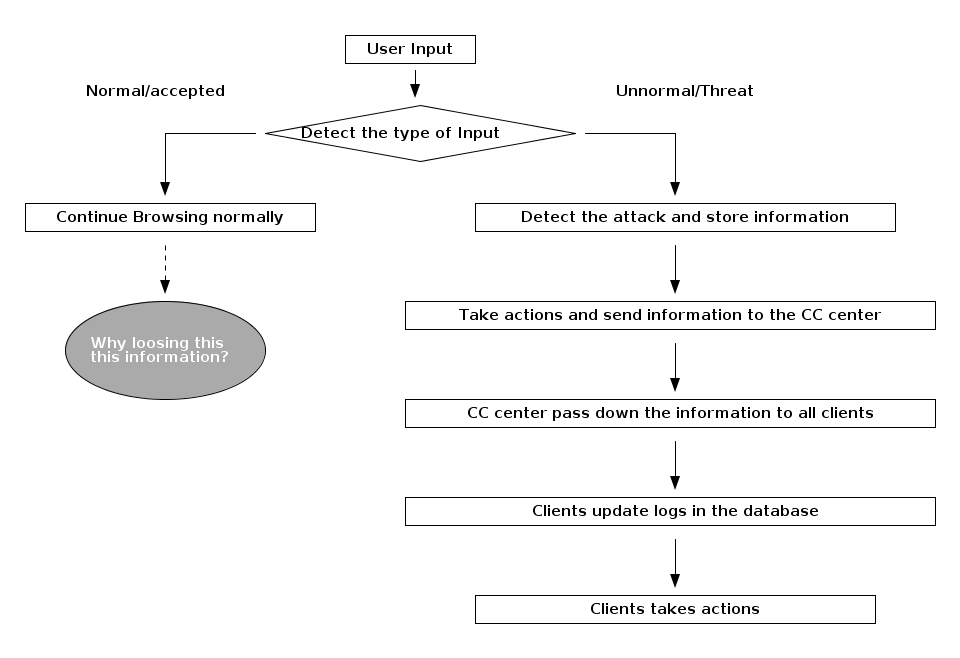
\includegraphics[width=15cm]{waf_mana}
    \caption{Zentralisiert~\cite{Manaseer2018}}
    \label{fig.topten}
  \end{center}
\end{figure}


% Oder: Der xxx Algorithmus

% Oder: Der yyy Algorithmus

% Zusammenfassung: ca. 0,5 Seiten
\section{Zusammenfassung}

\begin{neu}
  Anfang mit Aufnahme des Altenbestands, hinzufügen Entwicklungsumgebung, Test, etc

  Entwicklung Zentrale Steuerung

  Entwicklung ML Anteil
\end{neu}